\documentclass[11pt]{amsart}
\usepackage[margin=1in]{geometry}
\usepackage{amsmath,amssymb,amsthm}
\usepackage{hyperref}
\usepackage{graphicx}

\newtheorem{theorem}{Theorem}[section]
\newtheorem{metatheorem}[theorem]{Metatheorem}
\newtheorem{corollary}[theorem]{Corollary}
\newtheorem{proposition}[theorem]{Proposition}
\newtheorem*{claim}{Claim}

\theoremstyle{remark}
\newtheorem*{remark}{Remark}

\title{Off-line scattering resonances for the Hecke triangle orbifolds, \\
and what the generic scattering axioms cannot decide}

%% TODO (owner): authorship, ordering, affiliations, and whether
%% Prof. S. Koyama is invited as coauthor are owner decisions. Do not fill in
%% beyond the single listed author below.
\author{Saar Shai}
%% TODO (owner): affiliation.
%% TODO (owner): acknowledgements.
%% TODO (owner): Koyama mention -- see companion draft KOYAMA_LETTER_DRAFT.md.

\date{DRAFT --- \today. NOT SUBMITTED.}

\begin{document}

\begin{abstract}
For every finite integer $q \ge 3$ we prove that the scalar
trivial-character scattering determinant $\varphi_q$ of the one-cusp
Hecke triangle orbifold $G_q \backslash \mathbb{H}$ has infinitely many
nonreal zeros $\rho$ with $\Re\rho > 1/2$, and therefore infinitely
many multiplicity-matched scattering poles $1-\rho$ with
$\Re(1-\rho) < 1/2$. In particular every nonarithmetic finite Hecke
group $G_q$, $q \notin \{3,4,6\}$, has a scattering resonance strictly
off $\Re s = 1/2$.

We then isolate the hypotheses the proof actually consumes as an explicit
axiom list $A$ (meromorphic continuation of order at most two, the
functional equation $\varphi(s)\varphi(1-s)=1$, reality, a generalized
Dirichlet series with the Hejhal archimedean factor at $\kappa=1$,
finiteness and reality of the right divisor with strip confinement, a
polynomial vertical bound, and the exact critical-line modulus), and prove
a metatheorem: $A$ \emph{entails the negation} of the naive on-line rigidity
statement. No proof schema quantifying over all models of $A$ can place
all right-half-plane zeros on $\Re s = 1/2$; a schema that appears to do
so is refuted already by the modular case $\varphi_3$. We also show that
$A$ fails to decide the genuine RH-analogue $P_{\mathrm{line}}(3/4)$ in
at least one direction, unconditionally.

The moral is not new: since Davenport--Heilbronn (1936) it has been
Dirichlet-series folklore that a functional equation without an Euler
product does not force on-line zeros, and the Selberg class encodes that
folklore as an axiom. What was missing was a theorem-strength analogue on
the spectral/scattering side. This paper supplies one.
\end{abstract}

\maketitle

\section{Introduction --- the honest framing}

\subsection{What is claimed, in one paragraph}

Following the defensible framing fixed for this paper: the moral ---
functional equation without arithmetic does not force on-line zeros ---
has been Dirichlet-series folklore since 1936 and is codified in the
Selberg-class axioms. It had \textbf{no theorem-strength analogue on the
spectral/scattering side}, which is precisely why spectral programs
continued as though their setting were exempt. We supply that analogue: a
family of scattering problems with the full analytic apparatus and
provably infinitely many off-line resonances.

\textbf{Mandatory correction.} An earlier framing of this claim ended
``with arithmeticity as the exact discriminant.'' That clause is refuted
by our own results and is deleted here: the non-arithmeticity clause is
non-discriminating --- $q=3$ (arithmetic) has the same off-line property
--- and must never be used as an arithmeticity signature (see
Corollary~\ref{cor:blindness} below, which makes the blindness formal).
The introduction states the blindness explicitly rather than letting a
reader infer a dichotomy.

\textbf{Where the novelty actually sits.} The two-sided comparison ---
one theorem for the structure-rich side, one for the structure-poor side
--- already exists at theorem strength in the Dirichlet-series world:
Hardy (1914) \cite{Hardy1914} proves infinitely many zeros of $\zeta$ \emph{on} the line,
Davenport--Heilbronn (1936) produces zeros \emph{off} the line for a
function without an Euler product. But those two theorems speak about
\textbf{unrelated functions from different constructions}; the comparison
is made by the reader, not by a parameter. The defensible novelty here is
that this is the first \textbf{single-family} version of that comparison
in the geometric/spectral setting: one parameter $q$, one construction,
where a proven classification (Takeuchi's list of the arithmetic $G_q$ \cite{Takeuchi1977})
sits beside the present theorem, so the family itself splits. Nothing
stronger may be claimed: the split is a statement about the two
literatures meeting inside one family, \textbf{not} an arithmeticity
criterion --- the off-line conclusion of \S\ref{sec:law} holds for
arithmetic $q=3$ as well.

\subsection{Prior art, cited as prior art}

\begin{itemize}
\item \textbf{Davenport--Heilbronn (1936); Epstein zeta functions of
class number $>1$} \cite{DH1936}. The canonical negative control on the
Dirichlet-series side: a function with almost all the properties of
$\zeta$ except an Euler product, with zeros off the line. Cited as the
origin of the moral, not as something we extend.
\item \textbf{Beurling generalized primes} (Beurling 1937; the
Diamond--Zhang lineage) \cite{Beurling1937}. The series-side sibling
programme: invented number systems that keep part of the multiplicative
structure and ask which PNT-facts survive, with known failures of the
RH-analogue among them. Cited as classical companion context for the same
question asked one construction over; we make no specific claim about any
Beurling system and consume nothing from that literature.
\item \textbf{The Selberg class.} The Euler product is an axiom there
\emph{precisely because} of Davenport--Heilbronn. Our axiom list $A$ is
the spectral-side mirror of that codification.
\item \textbf{Conrey--Li (2000)} \cite{ConreyLi2000}. The methodological
precedent: a negative control that kills a named proof schema (de Branges
positivity). Our metatheorem is modelled on this argument shape.
\item \textbf{Sarnak, ``Problems of the Millennium: RH''} \cite{Sarnak2004}.
Three quotable positions: scepticism that generic self-adjointness is the
source of a proof; the Conrey--Li refutation of de Branges' positivity;
the separation of ``arithmetic $\pi$'' from ``transcendental $\pi$'' for
GRH.
\item \textbf{Hejhal, LNM 1001, Thm.\ 7.11 / Cor.\ 7.12 (pp.\ 577--579)}
\cite{Hejhal1983}. The \emph{printed partial antecedent}: for all
sufficiently large $N$, zeros and poles of $\varphi_N$ in any prescribed
rectangle touching the critical line. Weaker in $q$-range, stronger in
localization. Cited wherever novelty is framed.
\item \textbf{Selberg (1990), ``Remarks on the distribution of poles of
Eisenstein series''} \cite{Selberg1990}. The source of the $d=2$ counting
theorem consumed as (C), per Kelmer Remark 0.2. \textbf{Not read} by the
authors of the underlying notes; see the declarations of unread sources,
\S\ref{sec:unread}.
\item \textbf{Kelmer, arXiv:1402.4780} \cite{Kelmer2014}, \S4 --- the
complex-analytic proof template (torsion-free global setup; only the
template is reused).
\item \textbf{Friedman--Jorgenson--Smajlovi\'c, arXiv:2011.12795}
\cite{FJS2020}, \S\S2.1, 2.4 --- continuation, functional equation, divisor
list in orbifold generality.
\item \textbf{Venkov, Trudy Mat.\ Inst.\ Steklov 153 (1981), Thm.\ 3.5, p.\ 59}
\cite{Venkov1981} --- \textbf{not} the 1979 Uspekhi survey; reached only
through FJS.
\item \textbf{Mayer--M\"uhlenbruch--Str\"omberg} \cite{MMS2012}, transfer
operator for the Hecke triangle groups --- presentation and the one-cusp
statement.
\end{itemize}

\subsection{What is \emph{not} claimed}

\begin{itemize}
\item We do \textbf{not} claim there is no proof of RH without an Euler
product.
\item We do \textbf{not} claim the RH-analogue in this family is
unprovable, undecidable, or independent of anything.
\item We do \textbf{not} claim any arithmeticity criterion.
Corollary~\ref{cor:blindness} is a \emph{blindness} statement.
\item $P_{\mathrm{naive}}$ failing is a statement about a naive
formulation, not about RH.
\end{itemize}

\textbf{One scope sentence to forestall an apparent conflict (theta
group).} A reader who recalls Hejhal Theorem 7.11 may suspect tension with
axiom A7, because that proof turns on $|\varphi_\infty|\not\equiv1$ for
the theta group $G_\infty$. There is none: $G_\infty$ has two cusps and
therefore lies outside the scope fixed by A0 and by our standing
restriction to finite $q\ge3$ with one cusp.

\section{The LAW (main theorem)}
\label{sec:law}

\begin{theorem}[paper-level, unconditional]
\label{thm:law}
For every finite integer $q\ge3$, the scalar trivial-character
scattering determinant of the one-cusp Hecke triangle orbifold has
infinitely many nonreal zeros $\rho$ with $\Re\rho>1/2$, and therefore
infinitely many multiplicity-matched scattering poles $1-\rho$ with
$\Re(1-\rho)<1/2$. In particular, every nonarithmetic finite Hecke group
$G_q$, $q\notin\{3,4,6\}$, has a scattering resonance strictly off
$\Re s=1/2$.
\end{theorem}

Supporting count, in the form the existence conclusion needs:
\[
F_q(\tfrac12,T)=\frac{1}{4\pi}T^2\log T+O_q(T^2),
\]
finitely many total right zeros forcing the defining sum to be only
$O_q(T)$.

\textbf{Certified-as-absent, and stated as absent here.} No effective
first height; no $q$-uniform error; no machine formalization of the
analytic content; no project-specific Selberg-zeta normalization. These
remain OPEN and are not needed for the stated LAW.

\textbf{Three wording repairs.} $\varphi_q$ has no central divisor and
the normalization $L_q^*$ has the exactly simple zero at $s=1/2$; the
horizontal $O_q(\log T)$ term uses the right-edge normalization and the
Selberg--Titchmarsh argument as reproduced by Kelmer, not the modulus
bound alone; no explicit formula for the group-dependent linear
coefficient $A_q$ is consumed, only its existence.

\textbf{Consume-side warning.} Do \textbf{not} consume $A_q$, $B_q$, or
$C_q$ numerics from Kelmer --- his printed $B_\Gamma$ carries a spurious
$\log\pi$ and his $A_\Gamma$ assembly formula is wrong (see the erratum,
\S\ref{sec:erratum}).

\subsection{The two certified pins at $q=5$}
\label{sec:twopins}

Beside the LAW's infinitude statement, two individual Selberg-zeta zeros
of $G_5$ are interval-certified to contour standard (Arb argument
principle, directed rounding, winding $=1$ so each zero is simple).

\begin{theorem}[two pins; computer-assisted]
\label{thm:twopins}
$Z_{G_5}$ has zeros $s_1, s_2$ with
\[
\Re s_1\in[0.45389418007494470,\,0.45389618007494470], \qquad
\Im s_1\in[5.7635362417301305,\,5.7635382417301305];
\]
\[
\Re s_2\in[0.41054273549473627,\,0.41054473549473627], \qquad
\Im s_2\in[7.81976724701551188,\,7.81976924701551188].
\]
The closed real-part intervals are disjoint with separation
$\ge 0.04334944458020843$. Consequently the nonreal strip zeros of
$Z_{G_5}$ lie on \textbf{no single vertical line} $\Re s=c$, for any
$c\in\mathbb R$.
\end{theorem}

Sources: the first-pin assembly (pin 1, DECLARED 2026-08-15, five
adversarial rounds) and the second-pin assembly (pin 2, REFEREED ---
PROMOTED 2026-08-26; two cold seats, both PASS-WITH-CORRECTIONS,
corrections applied). The no-single-line consequence is
Corollary~\ref{cor:novertical} below; its logical core is
machine-verified (\S\ref{sec:machineverif},
\texttt{TwoPinNoLine.lean}). By the FJS completed-zeta divisor
classification (one cusp, scalar $\varphi_5$) and the Lean-verified
pole-to-zero reflection under $\varphi(s)\varphi(1-s)=1$, the pins
transport to two zeros $\rho_i=1-s_i$ of $\varphi_5$ with distinct real
parts in $(1/2,1)$ --- the witness of \S\ref{sec:metaIII} consumes.
Dependency standing: computer-assisted + citation-backed (FJS/MMS);
including the MMS $q=5$ heading caveat and the FJS p.\ 4 $k$-notation
caveat, both stated in full at their point of use below.

\section{The axiom list $A$ and the metatheorems}
\label{sec:metatheorems}

\subsection{The structures}

A \emph{Hecke-type scattering pair} is $M=(\varphi,\mathcal D)$ with
$\varphi$ meromorphic on $\mathbb C$ and
$\mathcal D=(d(n),g_n)_{n\ge1}$ its Dirichlet data. Write
$\mathfrak M(A)$ for the class of pairs satisfying A0--A7. Nothing in the
language of $A$ mentions $q$, a group, a surface, arithmeticity, or
$\zeta$.

\subsection{The axioms}

\begin{itemize}
\item[\textbf{A0}] (scalar, one channel, $\kappa=1$). $\varphi$ is a
$1\times1$ determinant; degree of singularity 1; the archimedean factor
carries $\kappa=1$.
\item[\textbf{A1}] (meromorphy and right-half-plane regularity).
$\varphi$ meromorphic on $\mathbb C$ of order at most 2, holomorphic in
$\Re s>1/2$ apart from finitely many poles.
\item[\textbf{A2}] (functional equation). $\varphi(s)\varphi(1-s)=1$.
\item[\textbf{A3}] (reality). $\varphi(\bar s)=\overline{\varphi(s)}$;
equivalently $d(n)\in\mathbb R$.
\item[\textbf{A4}] (generalized Dirichlet series, Hejhal archimedean
factor). For $\Re s>1$,
\[
\varphi(s)=\sqrt\pi\,\frac{\Gamma(s-\tfrac12)}{\Gamma(s)}\sum_{n\ge1}d(n)g_n^{-2s},
\]
with $0<g_1<g_2<\dots\to\infty$ discrete, $d(1)\neq0$, the series
absolutely convergent. \textbf{A4$^+$} (used only where flagged):
$d(n)>0$.
\item[\textbf{A5}] (right divisor: finiteness, reality of poles, strip
confinement --- D2-corrected form). In $\Re s>1/2$: finitely many real
zeros $\rho_i>1/2$ with multiplicity; every pole of $\varphi$ in
$\Re s>1/2$ is real and lies in $(1/2,1]$, and there are finitely many;
and every zero lies in a vertical strip. (The reality-of-poles clause is
used essentially.)
\item[\textbf{A6}] (vertical polynomial bound). For every $\varepsilon>0$
there is $C(\varepsilon)<\infty$ with
$|\varphi(\sigma+it)|\le C(\varepsilon)$ for $1/2\le\sigma\le3/2$,
$|t|\ge\varepsilon$.
\item[\textbf{A7}] (critical-line modulus). $|\varphi(1/2+it)|=1$ for
real $t$, in the exact-modulus form, not merely unitarity.
\end{itemize}

\textbf{Not in $A$, deliberately:} any Euler product, multiplicativity,
or Ramanujan bound; any group, surface, or spectral input beyond A0; any
$q$-uniformity; any effective first height; any arithmeticity.

\textbf{Note on strip confinement.} Strip confinement is not an
independent assumption: it is an immediate corollary of A4 via the
right-edge estimate $|L^*-1|<1$ for large $\Re s$.

\subsubsection{Where $\varphi_q$ sits}

$\varphi_q$ is \textbf{not} a member of the Selberg class. For $q=3$
this is unconditional and elementary: $\varphi_3=\Lambda(2s-1)/\Lambda(2s)$
has a pole at every $s=\rho/2$ with $\rho$ a nontrivial zero of $\zeta$,
so no $(s-1)^m\varphi_3(s)$ is entire, and $\varphi_3$ is unimodular on
$\Re s=1/2$, which no Selberg-class function is. For general $q$ the
frequencies $g_n$ are not integers, so even the Dirichlet-series axiom
fails as stated. To our knowledge $\varphi_q$ also lies outside the
known extensions of the class, but we have not attempted a systematic
check and make no classification claim.

\subsection{Breadth lemma}

$\varphi_q\in\mathfrak M(A)$ for every finite integer $q\ge3$, arithmetic
and non-arithmetic alike. Receipts are per-axiom, both sides; in five of
the nine rows the two columns are the same citation (A0, A4, A4$^+$, A6,
A7); A1, A2, A3, A5 carry distinct arithmetic-side derivations from
$\Lambda$. $A$ was not assembled by intersecting two separately verified
lists.

For $q=3$ the Dirichlet data is explicitly $d(n)=\phi_{\rm Euler}(n)$,
$g_n=n$, $d(1)=1$, giving
$\sum d(n)g_n^{-2s}=\zeta(2s-1)/\zeta(2s)=L^*_3(s)$. Hejhal's Lemma 7.3,
used in the A4$^+$ row, is printed for $N\ge4$ and does \textbf{not}
cover $q=3$; $q=3$ is covered by the direct positive-integer count.

\subsection{The two candidate rigidity statements}

\[
P_{\mathrm{naive}}: \ \varphi \text{ has no zero } \rho \text{ with }
\Re\rho>1/2 \text{ and } \Im\rho\neq0,
\]
\[
P_{\mathrm{line}}(c): \ \text{every zero } \rho \text{ with }
1/2<\Re\rho<1,\ \Im\rho\neq0, \text{ has } \Re\rho=c.
\]

This is the canonical definition of $P_{\mathrm{naive}}$ and must be used
everywhere; A5 explicitly permits finitely many \emph{real} right zeros,
so the ``no zeros at all'' reading is non-derivable for a second and
trivial reason.

\subsection{Metatheorem I}

\begin{metatheorem}
\label{met:I}
$A \models \neg P_{\mathrm{naive}}$. Every $M\in\mathfrak M(A)$ has
infinitely many zeros $\rho$ with $\Re\rho>1/2$, $\Im\rho\neq0$, and
hence by A2 infinitely many multiplicity-matched poles $1-\rho$ with
$\Re(1-\rho)<1/2$.

\textbf{Consequence (the no-go).} There is no valid derivation of
$P_{\mathrm{naive}}$ from $A$ --- not because $A$ is too weak, but
because $A$ proves its negation. Any argument that appears to derive
on-line rigidity in the sense of $P_{\mathrm{naive}}$ from meromorphic
continuation, the functional equation, critical-line unitarity, a
generalized Dirichlet series, and polynomial vertical growth
\textbf{contains an error}, and the error can be exhibited: \textbf{apply
the argument to $\varphi_3$}, where the failure is classical fact.
\end{metatheorem}

\emph{Proof sketch.} This is the LAW read as a statement about
$\mathfrak M(A)$ rather than about Hecke orbifolds. Every input is an
axiom: the right-edge estimate from A4; the Jensen/Littlewood rectangle
from A1, A5 (finitely many real right poles), A6 (horizontal edges), A4
(right edge to $+\infty$); the critical-line integral with leading
coefficient $1/4\pi$ from A7's exact modulus plus
$|\Gamma(\tfrac12+it)/\Gamma(it)|^2=|t|\tanh(\pi|t|)$; the divergence
step from A5 against $F(\tfrac12,T)=(1/4\pi)T^2\log T+O(T^2)$, with
strip confinement (A5) consumed at the divergence step to convert an
unbounded weighted sum into infinitely many zeros; strictness from the
vanishing Jensen weight at $\Re\rho=1/2$, independently from A2+A3+A7
forcing no divisor on the line at all; nonreality from A5; and reflection
from A2. No step consumes a group, a surface, arithmeticity, an Euler
product, or $q$.

\textbf{Status and the exact residual.} The unconditional form
$A\models\neg P_{\mathrm{naive}}$ is licensed by a genericity/transfer
addendum: the Sel90-bypass derivation cites only interface facts plus
classical ambient analysis, each a consequence of the corrected axiom
list, so the derivation transfers verbatim to an arbitrary
$M\in\mathfrak M(A)$. Residuals that remain, none of them a hypothesis on
$\varphi$: the rectangle identity is consumed only in the (J)-avg/H3
form; GAP-1 ((J)-sharp, remainder $O_q(\log T)$ at \emph{every} height)
and GAP-2 ((C) and (DIF)) still rest on Selberg 1990 and are absent from
the conclusion chain's signature.

\subsection{Metatheorem II}

\begin{metatheorem}[conditional on RH]
Assume RH. Then $A\nvDash\neg P_{\mathrm{line}}(3/4)$: the pair
$\varphi_3\in\mathfrak M(A)$ satisfies $P_{\mathrm{line}}(3/4)$. Hence
there is no valid derivation from $A$ of the failure of on-line rigidity
in its RH-analogue form.
\end{metatheorem}

The conditionality is unavoidable for this witness; we give no argument
that no other $M\in\mathfrak M(A)$ has unconditionally collinear
right-strip zeros.

\subsection{The RH calibration}

\begin{proposition}
$P_{\mathrm{line}}(3/4)$ holds for $\varphi_3$ if and only if RH.
Moreover $P_{\mathrm{naive}}$ fails for $\varphi_3$ unconditionally.
\end{proposition}

\emph{Proof.} From $\varphi_3(s)=\Lambda(2s-1)/\Lambda(2s)$: the zeros of
$\varphi_3$ in $\Re s>1/2$ are exactly $s=(1+\rho)/2$ for $\rho$ a
nontrivial zero of $\zeta$, a multiplicity-preserving bijection, all
nonreal, all with $1/2<\Re s<1$; and $\Re((1+\rho)/2)=3/4\iff\beta=1/2$.
Confirmed unconditionally and re-verified numerically to 20+ digits. The
closed form for $\varphi_3$ is a \textbf{not-read} standard citation
(Iwaniec, \emph{Spectral Methods of Automorphic Forms}, 2nd ed., \S3.4
\cite{Iwaniec2002}), corroborated twice inside our own bank.

\textbf{Why this matters.} The functional equation reflects about
$\Re s=1/2$, so $1/2$ is the \emph{symmetry} line; the zeros of the
underlying $\zeta$ are pushed to $\Re s=3/4$ by $w=2s-1$, so $3/4$ is the
\emph{rigidity} line. Writing ``on-line rigidity'' without saying which
line is the mistake this paper exists to catch.

By A2, $P_{\mathrm{line}}(3/4)$ for zeros is equivalent to all nonreal
scattering poles of the modular orbifold lying on $\Re s=1/4$ --- the
Faddeev--Pavlov / Lax--Phillips reading (both \textbf{not-read}
citations here \cite{FaddeevPavlov1972,LaxPhillips1976}; the equivalence
above does not depend on them).

\subsection{The decision table}

\begin{center}
\begin{tabular}{p{4.3cm}p{4cm}p{4.3cm}}
\hline
statement & relation to $A$ & status \\
\hline
$P_{\mathrm{naive}}$ & $A\models\neg P_{\mathrm{naive}}$ & PROVED, unconditional in the upgraded form; residuals GAP-1/GAP-2 outside the conclusion chain \\
$\neg P_{\mathrm{line}}(3/4)$ & $A\nvDash\neg P_{\mathrm{line}}(3/4)$ & PROVED, conditional on RH; witness $\varphi_3$; conditionality unavoidable for this witness \\
$P_{\mathrm{line}}(3/4)$ & $A\models P_{\mathrm{line}}(3/4)$? & SETTLED NO (2026-08-26) --- Metatheorem III gives $A\nvDash P_{\mathrm{line}}(3/4)$ unconditionally (was OPEN/RH-hard) \\
decidability of $P_{\mathrm{line}}(3/4)$ by $A$ & $A$ fails to decide it in at least one direction & PROVED UNCONDITIONALLY \\
$P_{\mathrm{line}}(c)$, every $c\in(1/2,1)$ & $A\nvDash P_{\mathrm{line}}(c)$ for every $c$ simultaneously & PROVED (Metatheorem III); computer-assisted/citation standing; witness $M_5$; unconditional, Sel90-free \\
\hline
\end{tabular}
\end{center}

The fifth row (2026-08-26) is the sharpest statement in the paper:
$A\nvDash P_{\mathrm{line}}(3/4)$ holds \textbf{unconditionally}, so the
third row's question is settled negatively without RH.

\subsection{Corollary --- arithmeticity-blindness, correctly glossed}

\begin{corollary}
\label{cor:blindness}
If $A\models S$ then $S$ holds for $\varphi_q$ for every finite $q\ge3$.
Consequently \textbf{no consequence of $A$} separates arithmetic
$q\in\{3,4,6\}$ from non-arithmetic $q$, and no $A$-only argument can
serve as an arithmeticity criterion.
\end{corollary}

\textbf{Mandatory accompanying sentence.} The Dirichlet \emph{data} is
\textbf{not} arithmeticity-blind: the structures are pairs
$(\varphi,\mathcal D)$ with the $g_n$ equal to the $|c|$-values, which
lie in $\mathbb Z[\lambda_q]$ and therefore encode $q$. An argument that
inspects the Dirichlet data --- still ``generic analytic machinery'' by
any ordinary reading --- is \textbf{not} covered by this corollary. Any
gloss of the form ``$A$ cannot separate the arithmetic members from the
non-arithmetic ones'' is refuted as written.

\subsection{Metatheorem III --- the former open problem, discharged}
\label{sec:metaIII}

The problem as originally posed: exhibit
$M=(\varphi,\mathcal D)\in\mathfrak M(A)$ and two nonreal zeros
$\rho_1,\rho_2$ with $1/2<\Re\rho_i<1$ and $\Re\rho_1\neq\Re\rho_2$. It is
now discharged by the \S\ref{sec:twopins} pins.

\begin{metatheorem}[fixed-witness quantifiers explicit]
\label{met:III}
There exists one $M_5=(\varphi_5,\mathcal D_5)\in\mathfrak M(A)$ ---
$\mathcal D_5$ the Hejhal/FJS Dirichlet data of the $q=5$ A4 receipt ---
such that for every $c\in(1/2,1)$, $M_5$ does not satisfy
$P_{\mathrm{line}}(c)$. Hence for every $c\in(1/2,1)$,
$A\nvDash P_{\mathrm{line}}(c)$: no member of the family
$P_{\mathrm{line}}(c)$ is derivable from $A$. One common countermodel
serves all $c$.

\textbf{Standing (part of the statement).} This result is
computer-assisted and citation-backed: it rests on the Arb interval
certificates for the two pins, the Lean-verified logical joints of
\S\ref{sec:machineverif}, and the cited published theorems --- the FJS
divisor classification (with the $k$-notation caveat of the dependency
ledger) and MMS Theorem 6.4 at $q=5$ (with the heading caveat stated
there). The scope is exactly the family $P_{\mathrm{line}}(c)$
--- not every statement informally describable as ``on-line rigidity.''
\end{metatheorem}

How each of the three original blockers fell: the Selberg-zeta pins
transport to $\varphi_5$ zeros $\rho_i=1-s_i$ by the FJS divisor
classification + one-cusp scalar specialization + the Lean-verified
reflection (\S\ref{sec:twopins}) --- an indirect, citation-backed
certificate the cold referee ruled sufficient; the second certified pin
(2026-08-26) supplies the distinct real part; and no synthetic
Davenport--Heilbronn countermodel is needed. Membership
$M_5\in\mathfrak M(A)$ is the breadth lemma at $q=5$.
\textbf{Sel90-independence.} The pin chain does not consume the LAW, so
Metatheorem III is free of the [Sel90, Lemmas 1, 2] residual carried by
Metatheorem I --- independence from that named engine, not from the
Selberg/scattering literature at large. Since RH is literally
$P_{\mathrm{line}}(3/4)$ for $\varphi_3$, Metatheorem III is the licensed
form of the slogan: any derivation of any $P_{\mathrm{line}}(c)$ from the
shared axioms alone contains an error, exhibitable by running it on
$M_5$.

\subsubsection{Proof of Metatheorem III --- the two-pin witness}
\label{sec:proofmetaIII}

Let $\mathcal D_5 = (d_5(n), g_{5,n})_{n\ge1}$ be the Hejhal/FJS
Dirichlet data used in the $q=5$ A4 receipt, and set
$M_5 = (\varphi_5, \mathcal D_5)$ --- the scalar scattering determinant
of the Hecke triangle group $G_5$ with its Dirichlet-series data.
$\mathfrak M(A)$ contains pairs, not bare functions.

\textbf{Membership.} $M_5 \in \mathfrak M(A)$ by the breadth lemma, at
the caveat level below.

\textbf{Two zeros, distinct real parts.} From the two certified
Selberg-zeta pins via the cited FJS divisor step, followed by the
Lean-verified order-preserving pole-to-zero implication under
$\varphi(s)\varphi(1-s)=1$ (the verified artifact is the nested file
\texttt{Scat1Lemma31Reflection.lean} --- Lean formalizes \emph{only} that
implication, not FJS, MMS, or $\varphi_5$ itself):
\[
\rho_1 = 1-s_1:\ \Re \in [0.54610381992505530,\ 0.54610581992505530],\quad
\Im \in [-5.7635382417301305,\ -5.7635362417301305];
\]
\[
\rho_2 = 1-s_2:\ \Re \in [0.58945526450526373,\ 0.58945726450526373],\quad
\Im \in [-7.81976924701551188,\ -7.81976724701551188].
\]
No conjugation enters: $\rho_i = 1-s_i$. Both nonreal (imaginary
intervals strictly negative), both real-part intervals strictly inside
$(1/2,1)$, closed-interval separation exactly $0.04334944458020843>0$,
hence $\Re\rho_1\neq\Re\rho_2$ certified.

For any fixed $c$, at least one of $\Re\rho_1,\Re\rho_2$ differs from
$c$, so a certified zero of $\varphi_5$ violates $P_{\mathrm{line}}(c)$.
Consequently no derivation from $A$ alone can establish any member of
the family $P_{\mathrm{line}}(c)$ --- the genuine RH-analogue family, not
merely $P_{\mathrm{naive}}$.

The Lean file \texttt{TwoPinNoLine.lean} additionally machine-verifies
the pure logical core (\texttt{no\_common\_line}: two distinct-real-part
zeros refute every vertical line simultaneously; exact gap
$4334944458020843/10^{17}$; disjointness; distinct-$\Re$), sorry-free,
axioms \texttt{[propext, Classical.choice, Quot.sound]}.

\textbf{Why this route is free of the Sel90 debt.} Metatheorem I
consumes the LAW, which carries the undischarged [Sel90, Lemmas 1, 2]
citation. This exhibition does \textbf{not} consume the LAW: the pin
chain is contour certificates (machine) + the Hilbert$\to$Banach
transport R5 + MMS Theorem 6.4 + whole-box $K_s$ exclusion + FJS divisor
+ Lean reflection core; the membership proof is the breadth lemma's
row-by-row Hejhal/FJS/MMS receipt table. Independence means the named
[Sel90, Lemmas 1, 2] engine is absent --- the route still cites other
published Selberg/scattering results and is \textbf{not} citation-free.

\textbf{Dependency ledger (carried caveats).}
\begin{itemize}
\item A5 flag superseded; A4 discreteness source-established by FJS
Thm.\ 2.1 (enumeration = corroboration); A1/A6 Hejhal/FJS transcriptions
cold re-extracted, not machine-checked quotations; width-one
normalization changes $\varphi$ by the zero-free factor $c^{1-2s}$
(functional equation and divisor preserved; disclosed).
\item \textbf{MMS $q=5$ heading inconsistency}: eq.\ (34) heading prints
``$q=2h_q+3>5$'' while the paper's general odd-$q$ incidence formulas,
Lemma 6.3, Theorem 6.4, and the explicit $q=5$ functional equation use
odd $q\ge5$; the $q=5$ identification rests on the general incidence
formula ($h_q=1$ specialization independently checked against the
three-row engine code). Any use of MMS Theorem 6.4 at $q=5$ must carry
this internal heading inconsistency.
\item \textbf{FJS p.\ 4 notation inconsistency}: immediately after
defining $k = \sum_j \dim V_j$ (degree of singularity, $=1$ here), FJS
prints ``$k=0$'' in a sentence evidently colliding with automorphic-weight
notation; Theorem 2.1 and the divisor formulas retain the
degree-of-singularity parameter. Does not alter the set-level divisor
classification; disclosed wherever FJS is cited as the scalar-specialization
source.
\item Both pin assemblies are computer-assisted; the FJS bypass is an
INDIRECT, citation-backed $\varphi_5$ zero certificate (no direct
evaluator of $\varphi_5$ exists); the cold referee ruled that closure of
this open problem requires zeros of $\varphi$, not a specified
certification technology, so this meets the standard.
\end{itemize}

\subsection{A worked audit --- how to apply Metatheorem I to a published construction}

A no-go of this kind is only useful if a reader can run it. This
subsection runs it once, in full, on a named construction from the
literature, so the procedure and --- equally important --- its limits
are both visible.

\textbf{Ledger discipline, binding on every sentence below.}
Metatheorem I licenses exactly one form of conclusion: \emph{any
derivation of $P_{\mathrm{naive}}$ whose every step is available in an
arbitrary $M\in\mathfrak M(A)$ contains an error, and the error is
exhibitable by running the derivation on $\varphi_3$.} It licenses
nothing about the correctness of any particular paper. Accordingly we do
\textbf{not} claim that the construction audited below is wrong, that its
Hamiltonian fails to exist, that its self-adjointness claim is false, or
that its programme cannot succeed. The audit's only output is a
\textbf{burden statement}: name the step that is not available in a
general $M\in\mathfrak M(A)$. A construction that can name one is
untouched by this paper.

\subsubsection{The test case}

We use the Berry--Keating $xp$ lineage and, as its most visible recent
instance, Bender, Brody and M\"uller, ``Hamiltonian for the zeros of the
Riemann zeta function,'' Phys.\ Rev.\ Lett.\ \textbf{118}, 130201 (2017)
(arXiv:1608.03679) \cite{BBM2017}. As reported in that paper's abstract,
the authors construct a Hamiltonian whose eigenvalues, subject to a
boundary condition on the eigenfunctions, correspond to the nontrivial
zeros of $\zeta$; the classical limit reproduces the Berry--Keating $xp$
picture; the operator is not Hermitian in the given inner product but is
$PT$-symmetric with broken $PT$ symmetry, and the authors give a
\emph{heuristic} construction of a metric operator defining an inner
product in which the Hamiltonian would be Hermitian. The paper's own
closing statement of the gap is explicit and is the reason it is the
right test case: \textbf{a rigorous proof that this Hamiltonian is
self-adjoint would establish the Riemann hypothesis.} This line is
classified elsewhere in our bank as exposure class (b) with a (c) tail,
its open gap being ``precisely a \emph{generic} self-adjointness claim.''

We audit the \textbf{self-adjointness step only} --- the step that is
open --- and not the construction of the operator, which is manifestly
$\zeta$-specific. We have not verified the paper's internal details
beyond its abstract and our classification of it; every description
above is flagged ``as reported in [BBM17]'' and the audit is written
schematically so that it does not depend on those details.

\subsubsection{Step (i) --- what the argument uses about the target function}

The self-adjointness step, stripped to the properties of the target
function it consumes, uses (as reported in [BBM17] and in the
surrounding $xp$ literature):
\begin{enumerate}
\item that the target is a meromorphic function of one complex variable
with a reflection symmetry about a distinguished vertical line;
\item that its relevant divisor is discrete, of finite density in
horizontal strips, and confined to a vertical strip;
\item that the reflection symmetry acts on the divisor as an involution
pairing $\rho$ with its mirror image, together with the reality symmetry
pairing $\rho$ with $\bar\rho$;
\item that the boundary condition on the eigenfunctions is a scalar,
one-channel condition;
\item that the resulting spectral problem is unitary on the
distinguished line, in the sense that the associated
scattering/transfer quantity has modulus one there;
\item polynomial vertical growth in the closed strip, used to control
the asymptotic and the metric-operator series.
\end{enumerate}
The conclusion sought is that the eigenvalues are real, i.e.\ that the
divisor lies on the distinguished line.

\subsubsection{Step (ii) --- each item is a consequence of $A$ or of ambient analysis}

\begin{center}
\begin{tabular}{p{7.5cm}p{4.5cm}}
\hline
item & supplied by \\
\hline
1. meromorphy with reflection about a distinguished line & A1 + A2 \\
2. discreteness, finite strip density, strip confinement & A5, with strip confinement itself an A4 corollary; finite density in strips from A1 (order $\le2$) via Jensen \\
3. reflection and reality involutions on the divisor & A2 + A3 \\
4. scalar, one-channel boundary data & A0 \\
5. unitarity on the distinguished line & A7, in the stronger exact-modulus form \\
6. polynomial vertical growth in the closed strip & A6 \\
ambient toolkit (Stirling, Jensen/Littlewood, Phragm\'en--Lindel\"of, Schwarz reflection, subharmonicity) & classical analysis, model-independent \\
\hline
\end{tabular}
\end{center}

No item on the list mentions primes, an Euler product, multiplicativity,
a Ramanujan bound, a group, a surface, or arithmeticity. That is the
substance of the audit: the properties the self-adjointness step is
reported to use are all in $A$.

\subsubsection{Step (iii) --- the conclusion Metatheorem I licenses}

Suppose the self-adjointness step could be completed using only items
1--6 and ambient analysis. Then the completed argument is a derivation,
from premises each of which holds in every $M\in\mathfrak M(A)$, of the
statement that the divisor in the right half-plane lies on the
distinguished line --- that is, of $P_{\mathrm{naive}}$. By
Metatheorem~\ref{met:I}, $A\models\neg P_{\mathrm{naive}}$. Hence such a
completion is impossible, and any argument that appears to achieve it
contains an error. Moreover the error is \textbf{exhibitable}, and
cheaply: instantiate the argument at
$M=(\varphi_3,\mathcal D_3)\in\mathfrak M(A)$, where items 1--6 all hold
and the conclusion is false as classical fact; the first step of the
argument that fails there is the step that was never available.

The burden this places is therefore precise and small: \textbf{name the
step of the self-adjointness argument that is not available for a
general $M\in\mathfrak M(A)$} --- equivalently, the step at which
$\zeta$-specific arithmetic re-enters. If such a step can be named, the
argument is untouched by this paper and has merely been disciplined. If
it cannot, the argument is incomplete in a way that no amount of
additional analytic rigour will repair.

\subsubsection{What this audit does \emph{not} establish --- four explicit weakenings}

\begin{enumerate}
\item \textbf{No refutation of [BBM17].} We do not claim the
construction is wrong. The audit's conclusion is conditional on the
self-adjointness step being completable from items 1--6 alone, which is
precisely what is open. Nothing here bears on the correctness of the
Hamiltonian, the $PT$ analysis, or the heuristic metric.
\item \textbf{The construction \emph{is} $\zeta$-specific; only the open
step is audited.} The operator in [BBM17] is built from $\zeta$-data, so
the programme as a whole is not an $A$-only schema. If the metric
operator's rigorous construction turns out to consume the Euler product,
the explicit formula over primes, or any other arithmetic input, then
the audit does not bite, and we do not assert that it does.
\item \textbf{Items 1--6 are our reconstruction, not the paper's own
hypothesis list.} We have not read a rigorous statement of the intended
self-adjointness argument, because none is published; we reconstruct the
properties it would use from the abstract and from the $xp$ literature.
A published argument using a property outside $A$ escapes the audit
automatically.
\item \textbf{The transfer to $\mathfrak M(A)$ requires the schema to be
restatable.} Metatheorem I quantifies over Hecke-type scattering pairs;
an operator-theoretic argument bites only once it has been restated as a
statement about $(\varphi,\mathcal D)$. Where a construction resists that
restatement, the audit is inapplicable rather than inconclusive. We
record this as a genuine limitation of the method, not as a formality.
\end{enumerate}

A fifth caveat is inherited from Corollary~\ref{cor:blindness}: an
argument that inspects the \textbf{Dirichlet data} $\mathcal D$ --- the
$g_n$, which lie in $\mathbb Z[\lambda_q]$ and encode $q$ --- is still
``generic analytic machinery'' by any ordinary reading, and is
nonetheless outside the reach of the arithmeticity-blindness corollary.
The audit above must be read as covering arguments that use $\varphi$
and the axioms, not arguments that mine $\mathcal D$.

\section{Appendix A (summary) --- the Jensen/Littlewood rectangle, re-derived}

Purpose: self-containedness. The rectangle identity (J) that the
counting argument consumes is normally imported from Selberg 1990,
Lemmas 1 and 2, reached only through Kelmer's (4.20). Appendix A
re-derives it from the standard complex-analytic toolkit and the
interface facts already used.

\begin{center}
\begin{tabular}{p{2.2cm}p{7.3cm}p{3.5cm}}
\hline
form & statement & status \\
\hline
(J)-sharp & rectangle identity with remainder $O_q(\log T)$ at
\textbf{every} $T$ & PARTIALLY re-derived --- one residual, GAP-1, a
pointwise negative-part bound at height $T$ \\
(J)-avg & same identity, remainder $O_q(\log T)$ for \textbf{some}
$T^*\in[T-1,T]$ & RE-DERIVED, unconditional on the banked inputs \\
H3 & $F_q(1/2,T)=(1/4\pi)T^2\log T+O_q(T^2)$, per-$q$, both halves &
RE-DERIVED from (J)-avg plus monotonicity of $F_q$ \\
\hline
\end{tabular}
\end{center}

Since the LAW's existence conclusion needs only H3, \textbf{the [Sel90]
citation is replaceable for the theorem of \S\ref{sec:law}}. It is
\emph{not} replaceable for the sharp asymptotic (C), which consumes
(J)-sharp through the finite-difference step; (C) does not appear in
this paper's conclusion chain.

Appendix contents in outline: Lemma A (orientation calibration of the
$\Gamma$-integral), Lemma B / (LW$\infty$) with the $1/\pi$, Lemma C (the
crux --- the potential $P(s)=-\int_s^\infty\log L^*$ has purely
imaginary jumps across the cuts, so $\Re P$ is continuous and
branch-free; no zero count is used anywhere, hence no circularity), and
Lemma D (conformal sub-mean-value on a translated half-disc, with
$\kappa(R)$ independent of $T$ because $H=H_0+iT$ is a pure translate).
The referee reproduced Lemma C's numerics on independent code at
$\mathrm{dps}=30$, agreeing to $10^{-26}$--$10^{-32}$ at seven heights
including two where the divisor is empty and two straddling the first
zero ordinate $\gamma=7.06736257086735$.

\textbf{Honesty items.} GAP-1 blocks only (J)-sharp; the Fubini
justification is by compactness on the box for each fixed $T$, with no
uniformity in $T$ claimed or needed; the $3/2<\sigma<\sigma_1$ strip is
covered by the absolutely convergent series bound.

\subsection{Remark --- an erratum in Kelmer, arXiv:1402.4780, eq.\ (4.18)}
\label{sec:erratum}

\textbf{Printed as a short remark, framed as service to the
literature.} Kelmer's (4.18) evaluates its last term as
$\log|t\tanh(\pi t)/\pi|$, where in fact
$|\Gamma(\tfrac12+it)/\Gamma(it)|^2=t\tanh(\pi t)$ exactly. The $/\pi$
inside the logarithm injects a spurious $-\tfrac12\log\pi$, so the
printed constant $B_\Gamma=(-4\log\pi-1)/(8\pi)\approx-0.22198$ is
wrong. Direct numerical evaluation of
\[
\frac{1}{2\pi}\int_{-T}^{T}(T-|t|)\log|L^*(\tfrac12+it)|\,dt-\frac{1}{4\pi}T^2\log T,
\]
divided by $T^2$, gives $-0.2107732$ at $T=200$, $-0.2105234$ at
$T=1000$ and $-0.2104734$ at $T=5000$, converging to
$(-2\log\pi-3)/(8\pi)\approx-0.2104609172$. The printed $A_\Gamma$
assembly formula is likewise wrong; the corrected relation is
$A=a+2B$, the coefficient $D$ cancelling identically.

The constant identities of that correction --- the finite-difference
leading term, the identity $A=a+2B$ with $D$ cancelling, the corrected
constant, and its disequality from Kelmer's printed $B_\Gamma$ (which
reduces to $\log\pi\neq1$) --- are targets of
\texttt{LawSkeletonI.lean} (Aristotle dispatch v33) and are
machine-verified there, sorry-free and axiom-clean.

\textbf{What this remark does not do.} The argument of this paper
consumes \textbf{none} of Kelmer's $A_q$, $B_q$, $C_q$ constants (see the
consume-side warning of \S\ref{sec:law}), so nothing above is
load-bearing for any statement here. The erratum is reported because it
is in the printed literature, not because we depend on it.

\section{Machine verification}
\label{sec:machineverif}

\subsection{How the claims of this paper were checked}

\textbf{Documentation of process, not a claim of method.} Comparable
verification pipelines exist elsewhere; nothing in this subsection is
offered as a methodological novelty. It is recorded only so a referee
can see what was done.

\begin{itemize}
\item \textbf{Cold adversarial refereeing.} Every load-bearing claim
passed at least one cold adversarial referee pass on an independent
lineage, with re-derivation rather than transcription: the LAW twice,
the metatheorem twice, and the Jensen/Littlewood re-derivation once.
\item \textbf{Independent numerics.} The Appendix A crux was re-run on
separately written code at $\mathrm{dps}=30$, agreeing with the
author's values to $10^{-26}$--$10^{-32}$ (26--31 digits) at seven
heights, four of them never tested by the author.
\item \textbf{Hash-pinned primary sources.} Each consumed PDF is
recorded with its digest; e.g.\ arXiv:1402.4780 at sha256
\texttt{c15fb0c4d1d72cc1e09ee6c70532e27d835afd8a8e01a23668cdb6049f8d5030}.
Sources reached only through another author's transcription are
declared as such in \S\ref{sec:unread}.
\item \textbf{Machine verification of the combinatorial finish} in
Lean~4, axiom-clean and conditional on the named hypotheses, as detailed
below.
\item \textbf{Append-only corrections.} Every correction was applied as
a dated append-only block, leaving the superseded text in place, so the
full audit trail is recoverable in the project repository.
\end{itemize}

\subsection{The verified statement}

The combinatorial / real-analytic \textbf{finish} of the theorem of
\S\ref{sec:law} is machine-verified in Lean~4 (Mathlib), conditional on
named hypotheses H1--H5, in
\texttt{aristotle\_dispatch\_v33\_aristotle/LawSkeletonI.lean} (the
returned, sorry-free artifact; status line ``No \texttt{sorry} bodies
remain,'' with an independent local re-compile recorded). The verified
statement is: growth of the weighted Jensen count together with
finiteness of the real zeros implies infinitely many strictly off-line
zeros and their reflections. \textbf{No scattering-theoretic content is
machine-verified}: $\varphi_q$ has no Lean definition, and no spectral
theory, meromorphic continuation, Jensen/Littlewood rectangle, or
property of $\varphi_q$ is formalized. Those enter only as named
hypotheses.

Two pointer corrections that must be respected:
\begin{enumerate}
\item The \emph{dispatch} file \texttt{aristotle\_dispatch\_v33/LawSkeletonI.lean}
is \emph{not} the artifact: it carries 16 \texttt{sorry} occurrences and
states ``This file machine-verifies nothing.'' Cite the
\texttt{aristotle\_dispatch\_v33\_aristotle/} path.
\item Per the dispatch summary, rows S5 (the rectangle (J)) and H3
(\texttt{hgrowth}) are relabelled to PROVED (refereed 2026-08-23,
corrections D-1..D-3 applied), in the consumed (J)-avg form only. Scope
limits unchanged: no $q$-uniform constant, no effective first height, no
machine formalization of the analytic content. \textbf{H4 and H5 keep
their ``NOT proved here'' labels.}
\item The logical core of Metatheorem III / Corollary~\ref{cor:novertical} is
machine-verified in
\texttt{aristotle\_dispatch\_v34/project\_aristotle/TwoPinNoLine.lean}
(returned artifact; local re-elaboration ``Build completed successfully
(8034 jobs)''; four theorems --- \texttt{no\_common\_line}, exact
interval gap $4334944458020843/10^{17}$, disjointness, distinct real
parts --- sorry-free, axioms exactly
\texttt{[propext, Classical.choice, Quot.sound]}; statements
byte-identical to the dispatch). The same scope warning applies:
$\varphi_5$ has no Lean definition; FJS/MMS content is cited, not
formalized. The pole-to-zero reflection core is the v33 nested artifact
\texttt{Scat1Lemma31Reflection.lean} (root dispatch stub still carries
\texttt{sorry}; cite the nested file).
\end{enumerate}

\subsection{Data availability}

\textbf{Draft paragraph, to be finalized at submission.} All material
supporting this paper is archived in the project repository: the Lean~4
sources and their compilation logs; the interval-arithmetic certificates
and shard-level receipts of the localization computation
(\S\ref{sec:q8}), including the per-leaf certification records and the
cross-host determinism check; the numerical scripts and outputs
underlying Appendix A and the erratum of \S\ref{sec:erratum}, together
with the independently written referee code and its values; the dated,
append-only correction blocks and the full cold-referee reports for
every load-bearing claim; and the SHA-256 digests of every primary
source consumed.

%% TODO (owner, before submission): deposit a citable, immutable
%% snapshot -- Zenodo DOI or equivalent -- and replace this paragraph's
%% repository reference with the DOI. No such archive exists at the time
%% of drafting, and no data-availability claim may be made in a submitted
%% version until it does.

\section{Declarations of unread and transcribed sources}
\label{sec:unread}

\begin{itemize}
\item \textbf{Selberg 1990, Lemmas 1 and 2} --- the complex-analytic
engine citation, reached only through Kelmer's transcription of (4.20).
\textbf{Not read} by any author or referee of the underlying notes. Its
content is re-derived in Appendix A in the consumed form; GAP-1 and
GAP-2 still rest on it and are outside the conclusion chain.
\item \textbf{Selberg 1990} is also the correct attribution for the
$d=2$ counting theorem consumed as (C) (per Kelmer Remark 0.2); Kelmer's
own contribution is the $d\ge3$ generalization.
\item \textbf{Iwaniec, \S3.4} --- the classical closed form of
$\varphi_3$; declared not read, corroborated twice inside our bank.
\item \textbf{Venkov, Trudy Mat.\ Inst.\ Steklov 153 (1981), Thm.\ 3.5,
p.\ 59} --- reached only through FJS, never at source. The 1979 Uspekhi
survey is the wrong item.
\item \textbf{Hejhal \S7 and FJS} --- consumed through \texttt{pdftotext}
\textbf{transcriptions}, not verbatim quotations; the A1 (order $\le2$)
and A6 chains rest on these.
\item \textbf{Faddeev--Pavlov, Lax--Phillips} --- not read; cited for
context only.
\item Hejhal (7.2)--(7.5) are stated for the conjugated group with cusp
width 1 and $\varkappa\equiv1$; the normalization changes $\varphi$ only
by the zero-free factor $c^{1-2s}$, which preserves the divisor and the
functional equation. $A$ is stated for the conjugated normalization.
\end{itemize}

\section{Certified localization at $q=8$ --- depth-8 checker output}
\label{sec:q8}

The merged depth-8 campaign records the following bounded computational
facts:

\begin{itemize}
\item All 1024/1024 depth-8 leaves across 4 arcs have status
\texttt{PASS}, satisfy $q_{\rm Op}<1$, and satisfy all strict gates.
\item Cross-host determinism is pinned: Kaggle and local produced a
byte-identical record with $rH = 0.1892125248420895230\ldots$ and
$qOp = 0.3271992747911403256\ldots$.
\item The merged checkpoint was validated by the checker's own
\texttt{validate\_checkpoint\_records} routine.
\item Checker sha:
\texttt{6a9c1c3d7b28c2e0741a5e880d1b12d48066437ea03efcfd3cda90743f1fc3b0}.
\end{itemize}

\textbf{Mandatory scope caveat (verbatim from the merge report,
\texttt{does\_not\_mean}).} This is checker output, not a theorem. E1,
the $q=8$ MMS/Hilbert identification, $K_s$, analytic gates 5-6 and
continuation condition 8 of the 12-item ledger are untouched and remain
OPEN.

\begin{figure}[h]
\centering
%% FIG-TODO (FIG-1): Four overlaid histograms show the per-arc
%% distribution of qOp_upper, using common bins and one series for each
%% of the 256 leaves on arcs 0, 1, 2, and 3. Horizontal axis: qOp_upper.
%% Vertical axis: leaf count. Data source: brace-expanded receipt glob
%% research_notes/rh_goals_2026-08-14/lane_g/kaggle_q8_subdivision/
%% shard_receipts/d8/SHARD_a[0-3]_l{0-64,64-128,128-192,192-256}.json.
%% For each receipt, group by $.payload.arc and read the 64
%% interval-valued strings at $.payload.records[*].qOp_upper; the
%% redundant per-record arc check is $.payload.records[*].arc_index.
%% Draw a vertical reference line at 1/(1+sqrt(2)) ~= 0.41421, labelled
%% "square-box predictor," and annotate the observed qOp_upper range as
%% approximately 0.22-0.33. NOT YET RENDERED.
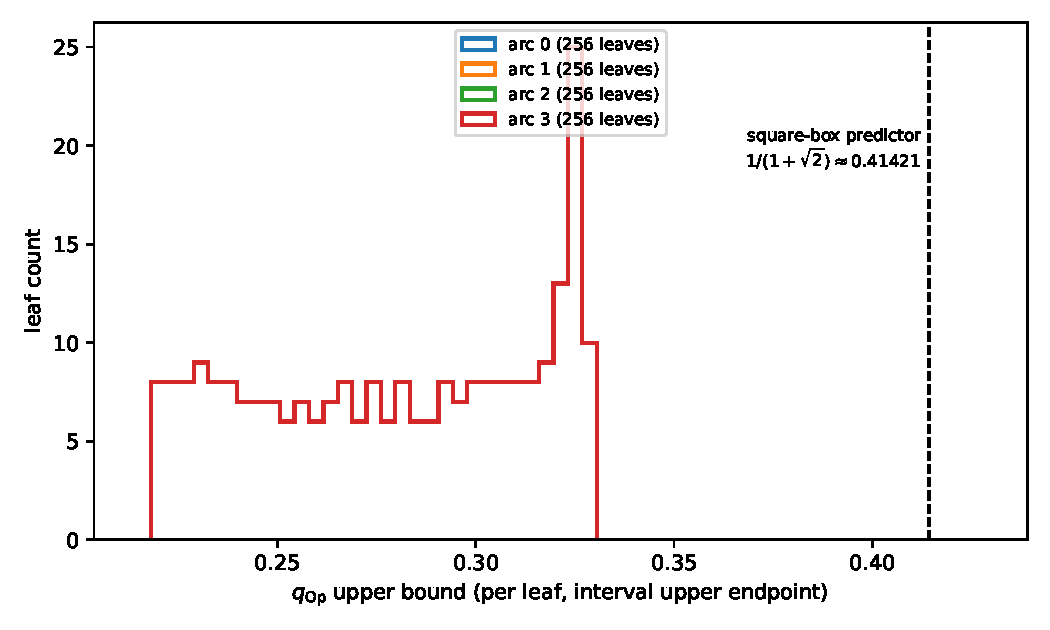
\includegraphics[width=0.85\linewidth]{fig1_qop_hist.pdf}
\caption{Per-arc distribution of \texttt{qOp\_upper} across the 1024
depth-8 leaves, arcs 0--3, with the square-box predictor
$1/(1+\sqrt2)\approx0.41421$ marked. \textbf{Not yet rendered.}}
\label{fig:qop}
\end{figure}

\section{Remark / outlook --- prime geodesics (NOT a theorem)}

\begin{remark}
The off-line resonances of \S\ref{sec:law} are Selberg-zeta zeros --- by
the Friedman--Jorgenson--Smajlovi\'c divisor description (subject to
the FJS $k$-notation caveat of the dependency ledger) they enter
\emph{reflected}, at $1-\rho$ with $\operatorname{Re}<1/2$. Their total
contribution to the prime geodesic counting formula is therefore
$O_q(x^{1/2}(\log x)^2)$: dominated by the main term and by every error
term under study. The correct statement is \emph{structural
bookkeeping}, not a constraint: the compact-surface divisor description
of Selberg-zeta zeros fails for every finite $q\ge 3$ (non-arithmetic in
particular; the property is non-discriminating --- $q=3$ has it too), by
an infinite, counted margin ($\gg_q T\log T$ reflected zeros below
height $T$) --- harmlessly for the PGT. Printed partial antecedent:
Hejhal LNM 1001, Thm.\ 7.11/Cor.\ 7.12 (large $N$).
%% Removed unresolved citation "Garbin--Jorgenson (2018)": no verified
%% title/venue could be confirmed; restore only with full bibliographic data.
\end{remark}

\textbf{Why the two sides are now asymmetric in kind.} On the
arithmetic side the divergence is already theorem-grade: improved error
terms in the prime geodesic theorem for arithmetic surfaces are proven
--- Luo--Sarnak (1995) \cite{LuoSarnak1995} and its successors --- by
exploiting the hidden multiplicative structure those surfaces carry. On
the non-arithmetic side the corresponding expectations have rested on
heuristics. The theorem of \S\ref{sec:law} supplies a \emph{structural}
statement on that side: infinitely many off-line scattering resonances,
in the frame the explicit formula uses. That is all it supplies.

\textbf{What must not be said here.} We derive no prime geodesic error
term, no $\Omega$-result (the LAW gives no information on the imaginary
parts, so no non-cancellation bound is reachable even in principle), no
effective first resonance height, and no $q$-uniform statement; the LAW
gives no effective first height at all. This remark is an outlook
paragraph naming a consumer, not a claim about the PGT.

\section{Corollary --- no single vertical line}

The results of \S\ref{sec:twopins}, translated into the Selberg-zeta
zero language of $G_5$ directly, give the following.

Let $G_5$ be the Hecke triangle group, $\lambda_5=2\cos(\pi/5)$ the
golden ratio; $X_5=G_5\backslash\mathbb H$ the non-arithmetic
finite-area hyperbolic orbifold; $Z_S=Z_{G_5}$ its Selberg zeta
function, meromorphically continued to $\mathbb C$. Write
\[
\Lambda := \{s\in\mathbb C : Z_S(s)=0\}, \qquad
\Lambda^\circ := \Lambda \cap \{0<\Re(s)<1,\ \Im(s)\neq0\}
\]
(the non-real strip zeros), and $L := \{s\in\mathbb C:\Re(s)=1/2\}$ (the
critical line). $\Lambda^\circ$ excludes the real-axis zeros (trivial
zeros from the identity contribution and the small-eigenvalue parameters
$s\in(1/2,1]$), which are present for every finite-area surface and
carry no information.

\begin{corollary}
\label{cor:novertical}
$\Lambda^\circ$ contains two zeros with certified real-part intervals
\[
\Re(s_1) \subset [0.45389418007494470,\ 0.45389618007494470], \qquad
\Re(s_2) \subset [0.41054273549473627,\ 0.41054473549473627],
\]
disjoint with closed-interval separation $\ge 0.04334944458020843>0$.
Hence \textbf{no single vertical line $V_c$ contains $\Lambda^\circ$, for
any $c\in\mathbb R$}: for each fixed $c$ at least one of the two
certified real parts differs from $c$.
\end{corollary}

\emph{Proof.} Immediate from Theorem~\ref{thm:twopins}: the certified
finite winding + closed-contour exclusion, together with the finite-section
identity, the Gohberg--Krein/Simon determinant comparison with machine
constants \cite{Simon1977,GrothendieckResume}, and the argument-principle
homotopy, place exactly one zero of $\det(1-L_{s,+})$ in each box; the
Hilbert$\to$Banach transport (R5) shows both boxes lie in the domain
$\Omega^*=\{\Re s>1/2\}\cup\{\Re s>0,\Im s>1\}$ where the Hilbert-space
and MMS Banach determinants agree; the whole-box $K_s$-divisor exclusion
shows neither box can have its zero cancelled by the $K_s$ factor; and
MMS Theorem 6.4 (subject to the $q=5$ heading caveat recorded in
\S\ref{sec:proofmetaIII}),
$Z_S = \det(1-L_{s,+})\cdot\det(1-L_{s,-})/\det(1-K_s)$, with
$\det(1-L_{s,-})$ analytic near each box, converts each determinant zero
into a zero of $Z_S$ of multiplicity at least that of the $+$ factor.
Since $\Im(s_1),\Im(s_2)\neq0$ and $0<\Re(s_i)<1$, both $s_1,s_2\in\Lambda^\circ$.
Disjointness of the real-part intervals with the stated separation is
exact decimal arithmetic, independently re-verified with Arb directed
rounding. For any fixed $c$, at least one $\Re(s_i)$ interval excludes
$c$, so $\Lambda^\circ\not\subset V_c$. $\blacksquare$

\textbf{Scope limits.} No claim is made that $\Lambda^\circ$ is disjoint
from $L$ in general, nor any density, counting, or distribution claim,
nor any family claim for $G_q$, $q\neq5$ (the family statement ``every
non-arithmetic Hecke group has an off-line resonance'' is a separate open
ticket, not a consequence of this corollary), nor any ``arithmetic
$\iff$ critical line'' law: the arithmetic Hecke triangle groups
$\{3,4,6\}$ form one commensurability class (one data point), and the
contrast noted here is descriptive of the data, not a proved equivalence.
The result is computer-assisted, resting on machine-certified Arb/Acb
interval receipts, Lean-proved abstract joints (Aristotle, axiom-clean),
cited published theorems (Simon \cite{Simon1977}, Grothendieck's
R\'esum\'e \cite{GrothendieckResume}, MMS Theorem 6.4 \cite{MMS2012}, standard
Selberg/scattering theory), and short self-contained paper-proofs. The
resonance \emph{interpretation} is citation-level standard theory, not
re-proved here; the determinant \emph{localization} does not depend on
it.

\section{Acknowledgments and authorship}

%% TODO (owner): acknowledgments, funding, collaborator credit, and the
%% authorship decision are left blank deliberately.

\section*{Drafting checklist before any submission}

\begin{itemize}
\item[$\square$] Owner decides authorship and whether to invite a coauthor.
\item[$\square$] Every ``NOT READ'' declaration of \S\ref{sec:unread} survives into the submitted text.
\item[$\square$] Hejhal Thm.\ 7.11 / Cor.\ 7.12 cited wherever novelty is framed.
\item[$\square$] The non-arithmeticity clause never presented as a discriminant.
\item[$\square$] \S\ref{sec:q8} either carries a completed, refereed certificate or is deleted.
\item[$\square$] Bombieri cited at most once, and not as a no-go.
\item[$\square$] Zenodo (or equivalent) deposit created and its DOI substituted into the data-availability paragraph.
\item[$\square$] The worked audit re-checked against the published text of every construction it names; the four weakenings survive into the submitted text, and no sentence asserts that a named paper is wrong.
\item[$\square$] A cold referee reads the assembled manuscript before submission.
\end{itemize}

\begin{thebibliography}{99}

\bibitem{DH1936} H.~Davenport and H.~Heilbronn, \emph{On the zeros of
certain Dirichlet series}, J. London Math. Soc. \textbf{11} (1936),
181--185. %% BIB-TODO: full page range / part II citation to confirm.

\bibitem{Beurling1937} A.~Beurling, \emph{Analyse de la loi asymptotique
de la distribution des nombres premiers g\'en\'eralis\'es}, Acta Math.
\textbf{68} (1937), 255--291. %% BIB-TODO: confirm Diamond--Zhang lineage citation detail.

\bibitem{ConreyLi2000} J.~B.~Conrey and X.-J.~Li, \emph{A note on some
positivity conditions related to zeta- and $L$-functions}, Internat.
Math. Res. Notices \textbf{2000}, no. 18, 929--940.

\bibitem{Sarnak2004} P.~Sarnak, \emph{Problems of the Millennium: the
Riemann Hypothesis}, Clay Mathematics Institute, 2004.

\bibitem{Hejhal1983} D.~A.~Hejhal, \emph{The Selberg Trace Formula for
$\mathrm{PSL}(2,\mathbb R)$, Vol.\ 2}, Lecture Notes in Mathematics 1001,
Springer, 1983. (Thm.\ 7.11 / Cor.\ 7.12, pp.\ 577--579.)

\bibitem{Selberg1990} A.~Selberg, \emph{Remarks on the distribution of
poles of Eisenstein series}, in Festschrift in honor of I.~I.~Piatetski-Shapiro,
Israel Math. Conf. Proc. \textbf{3} (1990), 251--278. %% BIB-TODO: confirm exact page range; NOT READ, cited via Kelmer.

\bibitem{Kelmer2014} D.~Kelmer, arXiv:1402.4780. %% BIB-TODO: confirm final published venue/title.

\bibitem{FJS2020} J.~S.~Friedman, J.~Jorgenson, L.~Smajlovi\'c,
arXiv:2011.12795. %% BIB-TODO: confirm final published venue/title.

\bibitem{Venkov1981} A.~B.~Venkov, Trudy Mat. Inst. Steklov \textbf{153}
(1981), Thm.\ 3.5, p.\ 59. %% BIB-TODO: confirm English title/translation; reached only through FJS, not read at source.

\bibitem{MMS2012} J.~Mayer, T.~M\"uhlenbruch, F.~Str\"omberg,
arXiv:0912.2236 (transfer operator for the Hecke triangle groups).
%% BIB-TODO: confirm final published venue/title.

\bibitem{Iwaniec2002} H.~Iwaniec, \emph{Spectral Methods of Automorphic
Forms}, 2nd ed., Graduate Studies in Mathematics 53, AMS, 2002. (\S3.4;
NOT READ, corroborated internally.)

\bibitem{FaddeevPavlov1972} L.~D.~Faddeev and V.~N.~Pavlov, \emph{Scattering
theory and automorphic functions}, Zap. Nauchn. Sem. LOMI \textbf{27}
(1972), 161--193. %% BIB-TODO: confirm citation detail; NOT READ, context only.

\bibitem{LaxPhillips1976} P.~D.~Lax and R.~S.~Phillips, \emph{Scattering
Theory for Automorphic Functions}, Annals of Mathematics Studies 87,
Princeton University Press, 1976. %% BIB-TODO: confirm citation detail; NOT READ, context only.

\bibitem{BBM2017} C.~M.~Bender, D.~C.~Brody, M.~P.~M\"uller,
\emph{Hamiltonian for the zeros of the Riemann zeta function}, Phys.
Rev. Lett. \textbf{118}, 130201 (2017), arXiv:1608.03679.

\bibitem{LuoSarnak1995} W.~Luo and P.~Sarnak, \emph{Quantum ergodicity
of eigenfunctions on $\mathrm{PSL}_2(\mathbf{Z})\backslash\mathbf{H}^2$},
Inst. Hautes \'Etudes Sci. Publ. Math. \textbf{81} (1995), 207--237.
(Contains the improved prime geodesic theorem error term for the modular
surface.)

\bibitem{Hardy1914} G.~H.~Hardy, \emph{Sur les z\'eros de la fonction
$\zeta(s)$ de Riemann}, C. R. Acad. Sci. Paris \textbf{158} (1914),
1012--1014.

\bibitem{Takeuchi1977} K.~Takeuchi, \emph{Arithmetic triangle groups},
J. Math. Soc. Japan \textbf{29} (1977), 91--106.

\bibitem{Simon1977} B.~Simon, \emph{Notes on infinite determinants of
Hilbert space operators}, Adv. Math. \textbf{24} (1977), 244--273. (Thm.\
4.2 with Lidskii Cor.\ 4.3.)

\bibitem{GrothendieckResume} A.~Grothendieck, \emph{La th\'eorie de
Fredholm}, Bull. Soc. Math. France \textbf{84} (1956), 319--384. (The Fredholm-determinant theory paper; Thm.~8 is consumed for the
determinant factorization. The 1955 tensor-norm \emph{R\'esum\'e} is a
different paper and is not the intended reference.)

\end{thebibliography}

\end{document}
